\chapter{Comportamiento dinámico y estabilidad}
El concepto de estabilidad y su análisis constituye unos de los aspectos claves para el estudio de los sistemas dinámicos. La estabilidad de un sistema esta estrechamente relacionada con su comportamiento dinámico y puede definirse de diversas maneras. En este capítulo nos centraremos en el análisis de los llamados puntos de equilibrio de un sistema y los estudiaremos de acuerdo con el concepto de estabilidad de Lyapunov. Además, incidiremos en otros aspectos de la estabilidad de los sistemas tales como la existencia de ciclos límite o el movimiento nominal. Empecemos pues por enunciar algunas definiciones de estabilidad.



\section{Estabilidad de un sistema dinámico}
Dado un sistema dinámico no forzado,
\begin{align}
\dot{x} = f(t,x) \label{eq: sis1}\\
y = g(t,x)
\end{align}

\begin{definition}[Estabilidad de las soluciones de un sistema dinámico]
Una solución $x(t;x_0)$ para la condición inicial $x(0) = x_0$ se dice que es estable si  $\exists R>0$ y  $ \exists r>0$ tal que, dada otra condición inicial $\hat x_0$ se verifica,
\begin{equation}
\|\hat x_0-x_0\|<r \Rightarrow \|x(t;\hat x_0) - x(t;x_0)\|<R, \forall t \geq 0
\end{equation}

En otro caso se dice que la solución es inestable 
\qed
\end{definition}

\begin{definition}[Estabilidad asintótica]
Una solución $x(t;x_0)$ para el sistema \ref{eq: sis1} se dice que es asintoticamente estable si es estable y además  $\exists r>0$, tal que dada otra condición inicial $\hat x_0$ se verifica,
\begin{equation}
\|\hat x_0-x_0\|<r \Rightarrow \lim_{t \to \infty}\|x(t;\hat x_0) - x(t;x_0)\|=0
\end{equation}

es decir, cualquier solución con condición inicial próxima  a $x(t;x_0)$ converge a $x(t;x_0)$
\qed
\end{definition}

\begin{definition}[Estabilidad marginal]
Una solución que es estable, pero asintóticamente estable, se denomina marginalmente estable
\qed
\end{definition}

\begin{definition}[Estabilidad exponencial]
Una solución $x(t;x_0)$ para el sistema \ref{eq: sis1} se dice que es exponencialmente estable estable si es estable y además  $\exists r>0$, tal que dada otra condición inicial $\hat x_0$ se verifica que existen $\alpha>0 , \sigma >0$, tales que,
\begin{equation}
\|\hat x_0-x_0\|<r \Rightarrow \|x(t;\hat x_0) - x(t;x_0)\| \leq \|\hat x_0 - x_0\| \alpha e^{-\sigma t}
\end{equation}
\qed
\end{definition}

Por último indicar que cuando la estabilidad se cumple para cualquier condición inicial, $\hat x  \in \mathbb{R}^n$ la solución $x(t;x_0)$ se denomina \emph{globalmente} estable.


\subsection{Puntos de equilibrio} 
\begin{definition}[Punto de equilibrio] Dados un sistema dinámico definido por las ecuaciones,
\begin{align}
\dot{x} = f(x,u)\\
y = g(x,u)
\end{align}
donde $x \in \mathbb{R}^n$, $u \in \mathbb{R}^m$ e $y \in \mathbb{R}^l$. Se definen como puntos de equilibrio o puntos estacionarios los valores del vector de estados $\overline x$ y del vector de entradas $\overline u$ para los cuales el estado y, consecuentemente, la salida del sistema permanecen constantes,

\begin{align}
\dot{\overline x} \equiv 0 = f(\overline x, \overline u)\\
\overline y = g(\overline x,\overline u)
\end{align}
\qed
\end{definition}

Si el vector de estados no cambia, su derivada será cero. Por tanto, mientras no se altere el valor de la entrada, el sistema permanecerá en el mismo estado y el valor del vector de salidas permanecerá también constante. 

Podemos, a partir de esta definición, obtener algunas propiedades importantes de los puntos de equilibrio:
\begin{enumerate}
\item Una vez que un sistema alcanza un punto de equilibrio, permanece en él indefinidamente. (Todas las derivadas temporales de las componentes del vector de estado son cero.
\item Desde el punto de vista del control de sistemas, los puntos de equilibrio juegan un papel importante ya que representan condiciones de operación constante.
\item Un sistema dinámico puede tener uno o más puntos de equilibrio, o no tener ninguno. 
\end{enumerate}

\paragraph{Sistemas autónomos.} Para simplificar el estudio de la estabilidad, podemos empezar por considerar el casos de sistemas autónomos con entrada nula  $u = 0, \ \forall t$. La salida evoluciona a partir de un estado inicial $x_0\equiv x(t_0)$,

\begin{align}
\dot{x} = f(x)\\
y = g(x)
\end{align}

\paragraph{Sistemas realimentados.} Del mismo modo, podemos considerar sistemas en los que la entrada es una función directa del valor de los estados; $\textbf{u}= \textbf{c(x)}$. Hablaremos entonces de un \emph{sistema realimentado}. A efectos de análisis de la estabilidad del sistema, no hay diferencia entre un sistema realimentado y un sistema autónomo,
\begin{align}
\dot{x} = f(x,c(x)) = \bar{f}(x)\\
y = g(x,c(x)) = \bar{g}(x)
\end{align}
El nombre de sistema realimentado, proviene de considerar que se están \emph{realimentando} los estados en la entrada del sistema. El concepto de realimentación constituye uno de los pilares de los sistemas de control. La figura \ref{fig:rea}, muestra esquemáticamente este concepto.

\begin{figure}
\centering
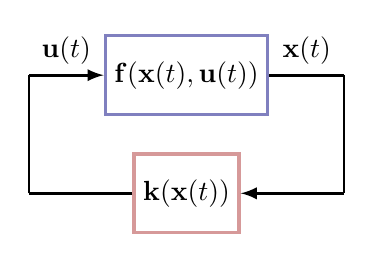
\begin{tikzpicture}
\draw(0,0) node(p)[rectangle, minimum height=10mm, minimum width=10mm,align=center, very thick, draw = blue!50!black!50]{$\mathbf{f}(\mathbf{x}(t),\mathbf{u}(t))$}

(0,-1.5) node(c)[rectangle, minimum height=10mm, minimum width=10mm,align=center ,very thick,draw = red!60!black!40]{$\mathbf{k}(\mathbf{x}(t))$};

\draw[line width = 1pt](p)--(2,0)node[midway,above]{$\mathbf{x}(t)$};
\draw[line width = 1pt](2,0)--(2,-1.5);
\draw[line width = 1pt, -latex](2,-1.5)--(c);
\draw[line width = 1pt](c)--(-2,-1.5);
\draw[line width = 1pt](-2,-1.5)--(-2,0);
\draw[line width = 1pt, -latex](-2,0)--(p)node[midway,above]{$\mathbf{u}(t)$};

\end{tikzpicture}

\caption{Esquema general de un sistema realimentado}\label{fig:rea}
\end{figure}

\section{Estabilidad de Lyapunov}
 En esta sección vamos a centrarnos en el estudio de la estabilidad de los puntos de equilibrio. 

Habitualmente, cuando se trata de la estabilidad de los puntos de equilibrio se suele hablar de estabilidad en el \emph{sentido} de Lyapunov. Aleksandr Mikhailovich Lyapunov un matématico ruso, de finales del siglo XIX, que estableció los fundamentos de la teoría de la estabilidad que ahora lleva su nombre.

Un punto de equilibrio de un sistema dinámico es \emph{estable} si toda  solución que comienzan cerca del punto de equilibrio permanece cercana al punto de equilibrio; en otro caso, el punto de equilibrio es inestable. Es \emph{asintóticamente estable} si toda solución que empieza próxima al punto de equilibrio no solo permanecen cerca del punto de equilibrio sino que tienden a él cuando el tiempo tiende a infinito.

Podemos relacionar directamente la estabilidad de un punto de equilibrio, con la estabilidad de las trayectorias de un sistema lineal definida en () i consideramos  un punto de equilibrio como una solución del sistema dinámico, cuya condición inicial es el propio punto de equilibrio: $x(t;\overline x) = \overline x$.

\subsection{Estabilidad de Lyapunov para sistemas autónomos}
Consideremos un sistema autónomo genérico,
\begin{equation}\label{eq: aut}
\dot x = f(x),
\end{equation}
donde $f(x): D\rightarrow \mathbb{R}^n$ es una función (localmente) lipschitziana desde un domino $D \subset \mathbb{R}^n$ a $\mathbb{R}^n$. Supongamos además que $\overline x \in D$ es un punto de equilibrio; es decir, $f(\overline x) = 0$. Lo que buscamos es un método para caracterizar el tipo de estabilidad de $\overline x$. En lo que sigue, y sin perdida de generalidad, consideramos que el punto de equilibrio es es origen de coordenadas $\overline x = 0$ \footnote{Siempre es posible hacer un cambio de coordenadas de modo que si $\overline x \neq 0$, $z = x-\overline x$; $\dot z = \dot x = f(x+\overline x) := g(z)$, donde $g(0)=0$.}.

\begin{definition} \label{def: est}
El punto de equilibrio x = 0 del sistema \ref{eq: aut} es:
\begin{itemize}
\item estable $\forall \epsilon > 0$ que cumpla:
\begin{equation*}
 \exists \delta =\delta(\epsilon)>0: \| x(0) \| < \delta \Rightarrow \| x(t)\| < \epsilon \ \forall t \ge 0
\end{equation*}
 
 \item Es inestable si no es estable.
 \item Es asintóticamente estable si es estable y además se puede elegir $delta$ de modo que,
\begin{equation*}
\| x(0)\| < \delta \Leftarrow \lim_{t \to \infty} x(t) = 0
\end{equation*}
\end{itemize}
\qed
\end{definition}

En 1892 Lyapunov propuso un método para analizar la estabilidad de un punto de equilibrio, basado en el análisis  una función $V:D\to \mathbb{R}$, continua y diferenciable en un entorno $D \subset \mathbb{R}^n$. En concreto, el método analiza la variación de la función $V$ a lo largo de las \emph{trayectorias} del sistema cuya estabilidad se quiere analizar, Podemos representar dicha variación empleando la derivada temporal de la función $V$
\begin{equation} \label{eq: dlyap}
\dot V(x) = \sum_{i=0}^{n}\frac{\partial V}{\partial x_i} \dot x_i = \sum_{i=0}^{n}\frac{\partial V}{\partial x_i} f(x) = \frac{\partial V}{\partial x}f(x)
\end{equation}

Es interesante hacer notar que, lógicamente, $\dot V$ depende del sistema que se desea analizar y que Si $\phi(t;x)$ es una solución del sistema \ref{eq: aut} , que empieza, como condición inicial, en estado $x$, para $t=0$ Entonces,
\begin{equation}
\dot V(x) =\left. \frac{d}{dt}V(\phi (t;x))\right|_{t=0},
\end{equation}
Por tanto, si $\dot V(x)$ es negativa, $V$ decrecerá a lo largo de la solución del sistema \ref{eq: aut}.

\begin{theorem}\label{th: lyap1}
Sea $x=0$ un punto de equilibrio para el sistema \ref{eq: aut} y $D \subset \mathbb{R}^n$ un dominio que contiene a $x=0$. Sea $V:D 	\to \mathbb{R}$ una función continua y diferenciable tal que,
\begin{equation}\label{eq: lyap1}
V(0) = 0\ y\ V(x) > 0\ en\  D-\{0\},
\end{equation}
\begin{equation}\label{eq: lyap2}
\dot V(x) \leq 0\ en\ D,
\end{equation} 
entonces $x=0$ es estable de forma local. Además, si
\begin{equation}\label{eq: lyap3}
\dot V(x) < 0 \ en\ D-\{0\},
\end{equation} 
Entonces $x(0)$ es asintóticamente estable de forma local.
\end{theorem}
\begin{proof}
Dado $\epsilon > 0$, elegimos $r \ in (0,\epsilon]$ tal que,
\begin{equation*}
B_r = \left\{ x \in \mathbb{R} \ |\  \|x\| \leq r \right\} \subset D.
\end{equation*}
Sea $\alpha =  \min_{\|x\| = r}V(x)$. Donde, $\alpha >0$ de acuerdo con \ref{eq: lyap1}. Tomamos ahora $\beta \in (0,\alpha)$ y construimos un nuevo dominio de modo que,
\begin{equation*}
\Omega_\beta = \left\{ x \in B_r \ |\  V(x) \leq \beta \right\}
\end{equation*}
Pero entonces $\Omega_\beta$ está en el interior de $B_r$.  Si no fuera así, sería posible encontrar un $p \in \Omega_\alpha$ que estaría situado en la frontera $B_r$. Pero en este punto $V(p) \ge \alpha > \beta$, lo que estaría en contradicción con la definición de $\Omega_\beta$. 

El conjunto $\Omega_\beta$ tiene la propiedad, de que cualquier trayectoria del sistema que empiece en $\Omega_\beta$  en $t=0$ permanecerá en $\Omega_\beta, \forall t \geq 0$; ya que, de acuerdo con \ref{eq: lyap2}
\begin{equation*}
\dot V \leq 0 \Rightarrow V(x(t)) \leq V(x(t)) \leq \beta, \forall t \geq 0.
\end{equation*}

Como $V(x)$ es continua y $V(0) = 0$,

\begin{equation*}
\exists \delta > 0\  |\  \|x\| \leq \delta \Rightarrow V(x) < \beta
\end {equation*}

la que implica que,
\begin{equation}
B_\delta \subset \Omega_\beta \subset B_r
\end{equation}
y
\begin{equation*}
x \in B_\delta \Rightarrow x(0) \in \Omega_\beta \Rightarrow x(t) \in B_r,
\end{equation*}
por tanto,
\begin{equation*}
\|x(0)\| < \delta \Rightarrow \|x(t)\|<r \leq \epsilon, \ t \geq 0
\end{equation*}

Lo cual demuestra que el punto $x=0$ es estable (ver definición: \ref{def: est}). 

Si además suponemos que se cumple \ref{eq: lyap3}, para demostrar que el sistema es asintóticamente estable, debemos probar que $x \to 0$ cuando $t \to \infty$; Condición que podemos reformular como, $\forall a >0, \exists T>0\ | \ \|x\| < a \ \forall t>T$. Pero, si repetimos nuestro razonamiento anterior, dato un valor $a>0$ siempre podremos encontrar un $b>0$ para el que se cumpla que $ \Omega_b \subset B_a$. Por tanto, es suficiente probar que $V$ alcanza el valor $0$ si nos movemos a lo largo de las trayectorias del sistema, $\lim_{t \to 0}V(x(t))=0$. Sabemos que $V(x(t))$ es monótona decreciente a lo largo de las trayectorias, y que está acotada inferiormente por cero.
\begin{equation}
\lim_{t \to 0}V(x(t)=c \geq 0
\end{equation}
Debemos demostrar que,  si se cumple \ref{eq: lyap3}, $c=0$. Vamos  demostrarlo por contradicción. Supongamos que $c>0$. Por continuidad de la función $V(x)$, $\exists d>0\ | \ B_d \subset \Omega_c$ pero entonces el límite $V(x(t))\to c>0$ implica que las trayectorias $x(t)$ se quedan fuera de la bola $B_d, \forall t \geq 0$. Si fijamos  un entorno $d \leq \|x\| \leq r$ exterior a $B_b$, $\dot V(x)$ deberá alcanzar un valor máximo, $-\gamma =\max_{d \leq \| x \| \leq r} \dot{V}(x)$. Además, por \ref{eq: lyap3} $-\gamma < 0$. Si integramos $\dot V$,
\begin{equation*}
V(x(t)) = V(x(0)) + \int_0^t \dot V(x(\tau))d\tau \leq V(x(0)) -\gamma t
\end{equation*}
Pero la expresión a la derecha del menor o igual, terminará por hacerse negativa, por lo que $c$ no puede ser mayor que 0.
\end{proof}
Algunas observaciones,
\begin{itemize}
\item Una función continua y diferenciable $V(x)$ que cumple las condiciones \ref{eq: lyap1} y \ref{eq: lyap2} recibe el nombre de función de Lyapunov.
\item La derivada $\dot V$, definida en la ecuación (\ref{eq: dlyap}) recibe el nombre de derivada de Lyapunov o derivada de Lie.
\item Una función $V(x)$ que satisface $V(0)=0$ y $V(x)>0$ para $x\neq 0$ en $D$, (\ref{eq: lyap1}), se dice que es definida positiva en $D$.Si la solo satisface $V(x)\geq 0$ para $x\neq 0$ en $D$, se dice que es semidefinida positiva en $D$.
\item Una función que cumple que $-V(x)$ es definida positiva/semidefinida positiva en $D$, se dice que es definida negativa/semidefinida negativa en $D$. Podríamos por tanto reescribir el teorema \ref{th: lyap1} diciendo que el origen es un punto de equilibrio estable, para un sistema dinámico si existe una función diferenciable definida positiva $V(x)$ tal que $\dot V(x)$ es semidefinida negativa, y es asintóticamente estable si $\dot V(x)$ es definida negativa.
\item El teorema \ref{th: lyap1} aporta condiciones suficientes para la estabilidad de un sistema; el hecho de no ser capaz de encontrar una función de Lyapunov para un sistema dado, no implica necesariamente que este sea inestable. 
\item Además, no es constructivo; indica que si existe una función de Lyapunov para el sistema, éste es estable, pero no indica cómo construir dicha función. 
\end{itemize}







\section{Principio de invarianza de LaSalle}

